% d8-system-anatomy.tex — KiteTurbineDynamics.jl
% Instructive anatomy of the V10 TRPT kite turbine
% Geometry from scripts/results/v10_campaign_50kw/best_design.json:
%   n_rings=10 intermediate (+ground+hub = 12 rings), n_lines=12 (12-gon),
%   rotor mask [1,4,7,10] from hub, r_bottom=2.0 m -> r_hub=2.89 m,
%   tether_length=67 m, target L/r ~ 3.0, blade scale 0.52 (hub) -> 0.10 (lowest rotor)
% (a) side elevation, wind left->right, beta = 30 deg (axial scale compressed)
% (b) view along shaft axis from the ground station
% Publication style: greyscale-safe, serif, terse labels.
\documentclass{article}
\usepackage[paperwidth=37.5cm,paperheight=14.5cm,margin=0.4cm]{geometry}
\usepackage{tikz}
\usetikzlibrary{calc,arrows.meta,patterns}
\usepackage{xcolor}
\begin{document}
\pagestyle{empty}
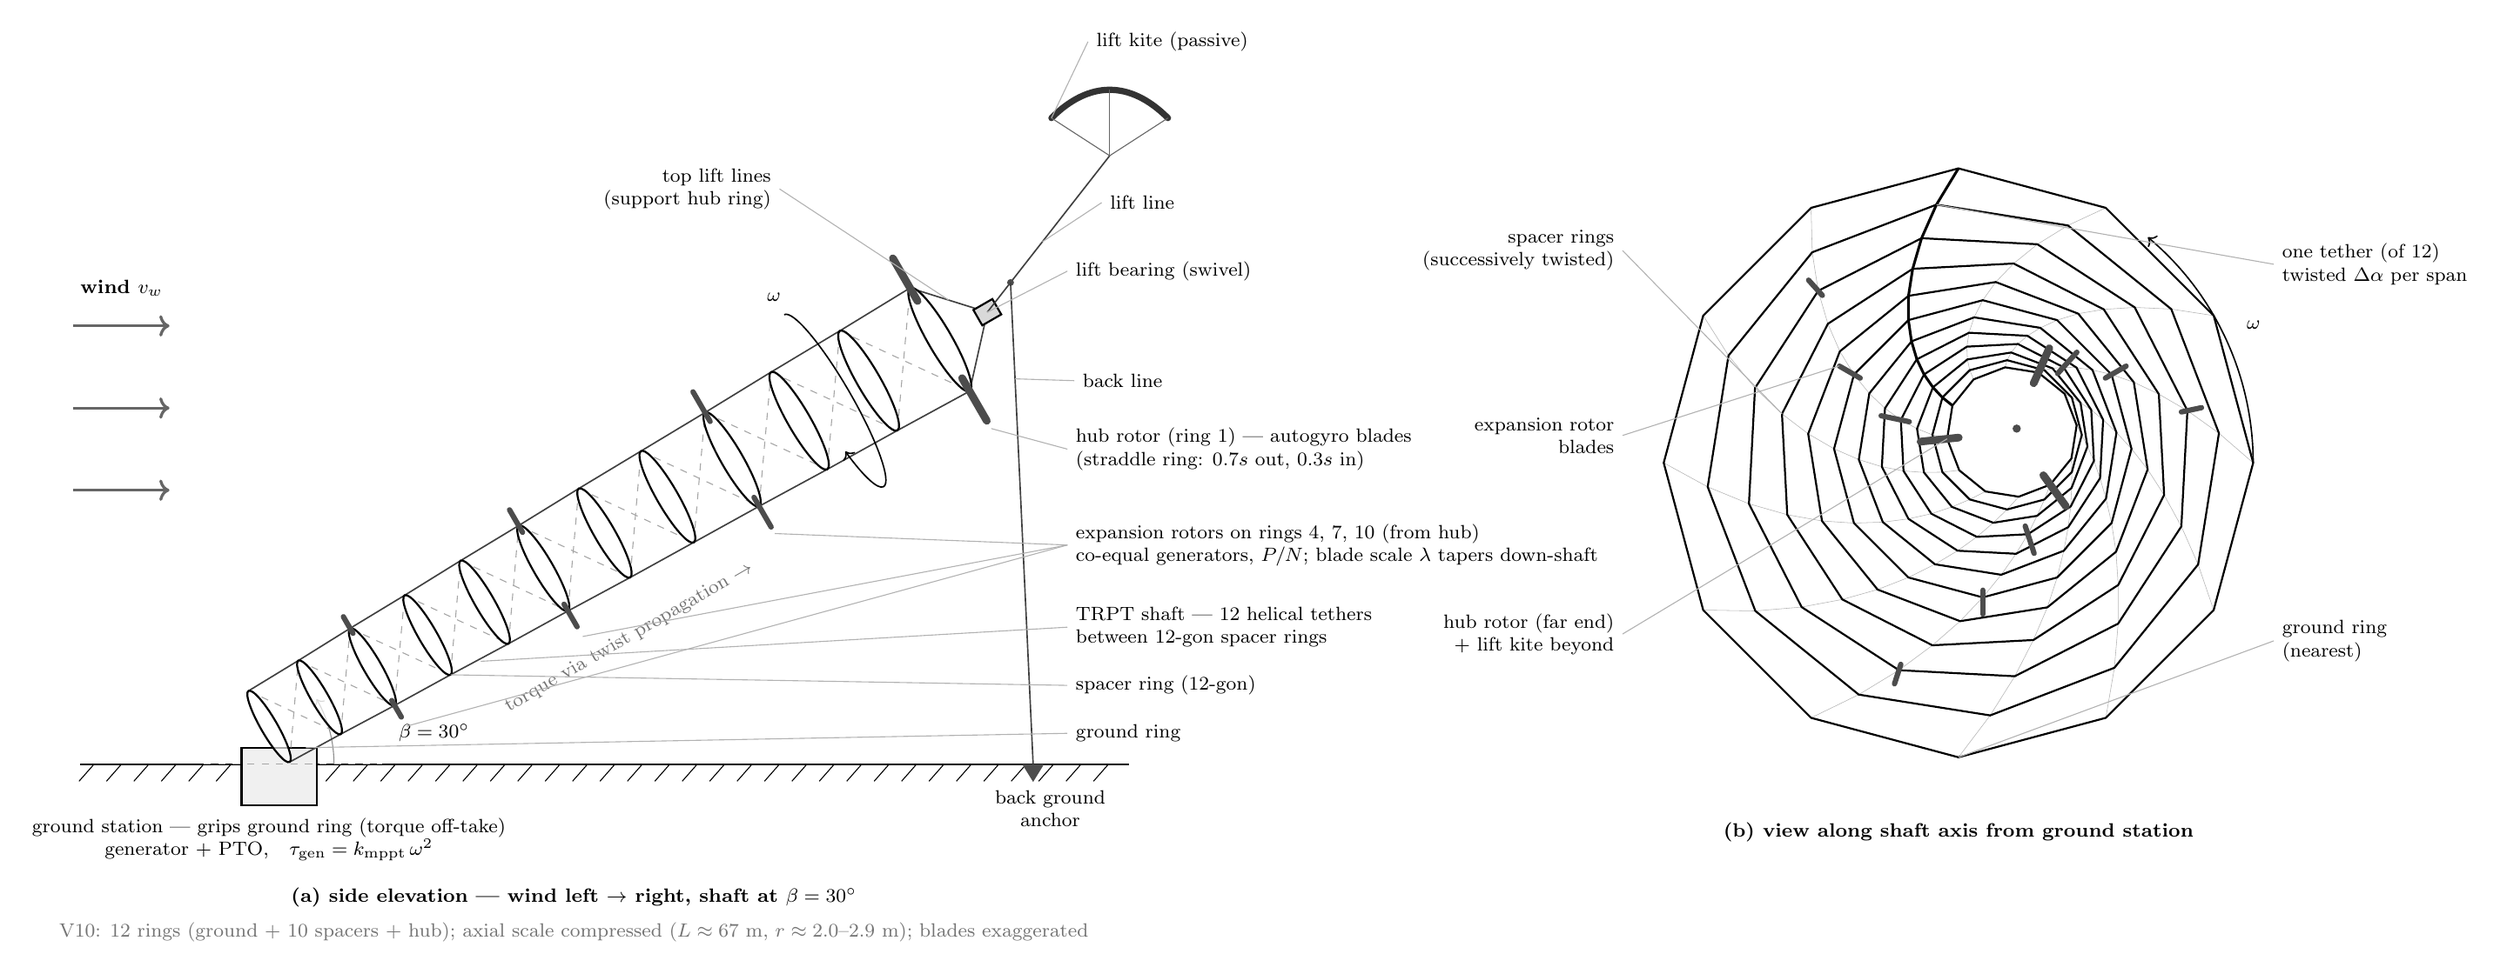
\begin{tikzpicture}[
  lbl/.style={font=\footnotesize},
  lblb/.style={font=\footnotesize\bfseries},
  leader/.style={gray!60, thin},
  ring/.style={black, thick},
  tether/.style={black!75, semithick},
  helix/.style={black!35, thin, dashed},
  blade/.style={line width=3.2pt, black!70, line cap=round},
  bladeB/.style={line width=2.2pt, black!70, line cap=round}
]

%%%%%%%%%%%%%%%%%%%%%%%%%%%%%%%%%%%%%%%%%%%%%%%%%%%%%%%%%%%%%%%%%%%%%%%
%% PANEL (a) — SIDE ELEVATION, wind left -> right, axis at beta=30deg
%%%%%%%%%%%%%%%%%%%%%%%%%%%%%%%%%%%%%%%%%%%%%%%%%%%%%%%%%%%%%%%%%%%%%%%
\begin{scope}
% ground
\draw[thick] (0.2,1.2) -- (15.5,1.2);
\foreach \x in {0.4,0.8,...,15.4} \draw[thin] (\x,1.2) -- (\x-0.22,0.95);

% ground station: grips the ground ring (torque off-take)
\draw[thick, fill=gray!12] (2.55,0.60) rectangle (3.65,1.44);
\node[lbl, align=center] at (2.95,0.10) {ground station --- grips ground ring (torque off-take)\\generator + PTO,\quad $\tau_{\mathrm{gen}}=k_{\mathrm{mppt}}\,\omega^2$};

% shaft axis origin (axis-ground intersection)
\coordinate (G) at (2.0,1.2);

% elevation angle beta
\draw[dashed, gray!70] (G) -- ++(2.6,0);
\draw[gray!90, ->] ($(G)+(0:1.9)$) arc (0:30:1.9);
\node[lbl, anchor=west] at ($(G)+(2.72,0.46)$) {$\beta=30^\circ$};

% 12 rings: ground (1), 10 intermediate, hub (12).
% Station s along axis (spacing prop. to r, constant L/r ~ 3.0, compressed),
% drawn radius r prop. to physical 2.0 -> 2.89 m.
% Rims: U = upper (120 deg), D = lower (-60 deg).
\foreach \i/\s/\r in {1/1.10/0.60, 2/1.95/0.62, 3/2.84/0.65, 4/3.77/0.67,
                      5/4.73/0.70, 6/5.72/0.72, 7/6.75/0.75, 8/7.81/0.77,
                      9/8.90/0.79, 10/10.03/0.82, 11/11.20/0.84, 12/12.40/0.87}{
  \coordinate (R\i) at ($(G)+(30:\s)$);
  \coordinate (U\i) at ($(R\i)+(120:\r)$);
  \coordinate (D\i) at ($(R\i)+(-60:\r)$);
}
\coordinate (BRG) at ($(G)+(30:13.20)$); % lift bearing (bridle apex)

% helix hints: dashed crossings on every span (12-line shaft)
\foreach \i [evaluate=\i as \j using int(\i+1)] in {1,...,11}{
  \draw[helix] (U\i) -- (D\j);
  \draw[helix] (D\i) -- (U\j);
}
% silhouette tether lines (upper & lower edges)
\draw[tether] (U1) -- (U2) -- (U3) -- (U4) -- (U5) -- (U6) -- (U7) -- (U8) -- (U9) -- (U10) -- (U11) -- (U12);
\draw[tether] (D1) -- (D2) -- (D3) -- (D4) -- (D5) -- (D6) -- (D7) -- (D8) -- (D9) -- (D10) -- (D11) -- (D12);

% top lift lines: hub-ring rim -> lift bearing (bridle supports hub ring)
\draw[tether] (U12) -- (BRG);
\draw[tether] (D12) -- (BRG);

% rings as edge-on ellipses (major axis perp. to shaft = 120deg)
\foreach \i/\r in {1/0.60, 2/0.62, 3/0.65, 4/0.67, 5/0.70, 6/0.72, 7/0.75, 8/0.77,
                   9/0.79, 10/0.82, 11/0.84, 12/0.87}{
  \begin{scope}[shift={(R\i)}, rotate=120]
    \draw[ring, fill=white, fill opacity=0.65] (0,0) ellipse ({\r} and {0.20*\r});
  \end{scope}
}

% rotors on mask rings [1,4,7,10] from hub = rings 12,9,6,3 from ground.
% Blades straddle the ring (0.3 span inboard / 0.7 outboard);
% blade scale tapers down-shaft: lambda 0.52 (hub) -> 0.10 (lowest rotor).
\foreach \p/\r/\s in {R3/0.65/0.28, R6/0.72/0.38, R9/0.79/0.50}{
  \draw[bladeB] ($(\p)+(120:{\r-0.3*\s})$) -- ($(\p)+(120:{\r+0.7*\s})$);
  \draw[bladeB] ($(\p)+(-60:{\r-0.3*\s})$) -- ($(\p)+(-60:{\r+0.7*\s})$);
}
\draw[blade] ($(R12)+(120:{0.87-0.22})$) -- ($(R12)+(120:{0.87+0.50})$);
\draw[blade] ($(R12)+(-60:{0.87-0.22})$) -- ($(R12)+(-60:{0.87+0.50})$);

% rotation arrow omega around the shaft between rings 10 and 11
\begin{scope}[shift={($(R10)!0.5!(R11)$)}, rotate=30]
  \draw[->, semithick] (0,1.45) arc (90:-150:{0.26} and {1.45});
\end{scope}
\node[lbl] at ($(R10)!0.5!(R11)+(120:1.75)$) {$\omega$};

% lift bearing (swivel) on axis
\begin{scope}[shift={(BRG)}, rotate=30]
  \draw[thick, fill=gray!30] (-0.16,-0.13) rectangle (0.16,0.13);
\end{scope}

% lift line + lift kite (canopy arc + bridle to confluence point K)
\coordinate (K) at ($(BRG)+(52:2.9)$);
\draw[tether] (BRG) -- (K);

% back line: taps lift line just above bearing, down to back ground anchor
\coordinate (BTAP) at ($(BRG)+(52:0.55)$);
\coordinate (ANC) at (14.1,1.2);
\fill[black!70] (BTAP) circle (0.05);
\draw[tether] (BTAP) -- (ANC);
\fill[black!70] ($(ANC)+(-0.16,0)$) -- ($(ANC)+(0.16,0)$) -- ($(ANC)+(0,-0.26)$) -- cycle;
\node[lbl, align=center] at (14.35,0.55) {back ground\\anchor};

\draw[line width=2.6pt, black!80, line cap=round]
  ($(K)+(-0.85,0.55)$) .. controls ($(K)+(-0.30,1.10)$) and ($(K)+(0.30,1.10)$) .. ($(K)+(0.85,0.55)$);
\draw[thin, black!60] (K) -- ($(K)+(-0.85,0.55)$);
\draw[thin, black!60] (K) -- ($(K)+(0,0.96)$);
\draw[thin, black!60] (K) -- ($(K)+(0.85,0.55)$);

% wind arrows
\foreach \y in {5.2,6.4,7.6} \draw[->, very thick, black!60] (0.1,\y) -- (1.5,\y);
\node[lblb] at (0.8,8.15) {wind $v_w$};

% torque-path annotation along shaft
\node[lbl, rotate=30, black!55] at ($(G)+(30:6.3)+(120:-1.5)$) {torque via twist propagation $\rightarrow$};

%% ---- labels (leaders) ----
\node[lbl, anchor=west] (Lkite) at (14.9,11.75) {lift kite (passive)};
\draw[leader] (Lkite.west) -- ($(K)+(-0.85,0.55)$);
\node[lbl, anchor=west] (Lline) at (15.1,9.4) {lift line};
\draw[leader] (Lline.west) -- ($(BRG)!0.45!(K)$);
\node[lbl, anchor=west] (Lbrg) at (14.6,8.4) {lift bearing (swivel)};
\draw[leader] (Lbrg.west) -- (BRG);
\node[lbl, anchor=east, align=right] (Ltop) at (10.4,9.6) {top lift lines\\(support hub ring)};
\draw[leader] (Ltop.east) -- ($(U12)!0.5!(BRG)$);
\node[lbl, anchor=west] (Lback) at (14.7,6.8) {back line};
\draw[leader] (Lback.west) -- ($(BTAP)!0.20!(ANC)$);
\node[lbl, anchor=west, align=left] (Lhub) at (14.6,5.8) {hub rotor (ring 1) --- autogyro blades\\(straddle ring: $0.7s$ out, $0.3s$ in)};
\draw[leader] (Lhub.west) -- ($(R12)+(-60:1.5)$);
\node[lbl, anchor=west, align=left] (Lexp) at (14.6,4.4) {expansion rotors on rings 4, 7, 10 (from hub)\\co-equal generators, $P/N$; blade scale $\lambda$ tapers down-shaft};
\draw[leader] (Lexp.west) -- ($(R9)+(-60:1.25)$);
\draw[leader] (Lexp.west) -- ($(R6)+(-60:1.15)$);
\draw[leader] (Lexp.west) -- ($(R3)+(-60:1.00)$);
\node[lbl, anchor=west, align=left] (Ltrpt) at (14.6,3.2) {TRPT shaft --- 12 helical tethers\\between 12-gon spacer rings};
\draw[leader] (Ltrpt.west) -- ($(R4)!0.5!(R5)+(-60:0.72)$);
\node[lbl, anchor=west] (Lring) at (14.6,2.35) {spacer ring (12-gon)};
\draw[leader] (Lring.west) -- (D4);
\node[lbl, anchor=west] (Lgr) at (14.6,1.65) {ground ring};
\draw[leader] (Lgr.west) -- ($(R1)+(-30:0.62)$);

\node[lblb] at (7.4,-0.75) {(a) side elevation --- wind left $\rightarrow$ right, shaft at $\beta=30^\circ$};
\node[lbl, black!55] at (7.4,-1.25) {V10: 12 rings (ground + 10 spacers + hub); axial scale compressed ($L\approx 67$ m, $r\approx2.0$--$2.9$ m); blades exaggerated};
\end{scope}

%%%%%%%%%%%%%%%%%%%%%%%%%%%%%%%%%%%%%%%%%%%%%%%%%%%%%%%%%%%%%%%%%%%%%%%
%% PANEL (b) — VIEW ALONG SHAFT FROM GROUND STATION (slight 3/4 offset)
%%%%%%%%%%%%%%%%%%%%%%%%%%%%%%%%%%%%%%%%%%%%%%%%%%%%%%%%%%%%%%%%%%%%%%%
\begin{scope}[shift={(27.6,5.6)}]

% ring i: apparent centre (cx,cy), apparent radius r, cumulative twist th (6 deg/span)
% i=1 ground ring (nearest, largest apparent) ... i=12 hub (farthest, smallest apparent)
\foreach \i/\cx/\cy/\r/\th in {1/0.000/0.000/4.30/0,  2/0.071/0.041/3.75/6,
                               3/0.142/0.082/3.27/12, 4/0.213/0.123/2.85/18,
                               5/0.284/0.164/2.49/24, 6/0.355/0.205/2.17/30,
                               7/0.426/0.245/1.89/36, 8/0.497/0.286/1.65/42,
                               9/0.568/0.327/1.44/48, 10/0.639/0.368/1.25/54,
                               11/0.710/0.409/1.09/60, 12/0.780/0.450/0.95/66}{
  \foreach \k in {0,...,11}{
    \coordinate (b\i-\k) at ($(\cx,\cy)+({\th+\k*30}:\r)$);
  }
}

% all 12 tethers, thin grey
\foreach \i [evaluate=\i as \j using int(\i+1)] in {1,...,11}{
  \foreach \k in {0,...,11}{
    \draw[black!30, very thin] (b\i-\k) -- (b\j-\k);
  }
}
% one highlighted tether path (k=3): the helix
\foreach \i [evaluate=\i as \j using int(\i+1)] in {1,...,11}{
  \draw[black, line width=1.1pt] (b\i-3) -- (b\j-3);
}

% polygons (draw far-to-near so near rings overprint)
\foreach \i in {12,11,10,9,8,7,6,5,4,3,2,1}{
  \draw[ring] (b\i-0) \foreach \k in {1,...,11} { -- (b\i-\k) } -- cycle;
}

% blades on rotor rings (3, 6, 9 from ground = expansion; 12 = hub), 3 shown per rotor,
% straddling the ring radially (0.3 in / 0.7 out)
\foreach \cx/\cy/\r/\th/\s in {0.142/0.082/3.27/12/0.30, 0.355/0.205/2.17/30/0.35,
                               0.568/0.327/1.44/48/0.42}{
  \foreach \a in {0,120,240}{
    \draw[bladeB] ($(\cx,\cy)+({\th+\a}:{\r-0.3*\s})$) -- ($(\cx,\cy)+({\th+\a}:{\r+0.7*\s})$);
  }
}
\foreach \a in {0,120,240}{
  \draw[blade] ($(0.780,0.450)+({66+\a}:{0.95-0.17})$) -- ($(0.780,0.450)+({66+\a}:{0.95+0.39})$);
}

% lift kite marker beyond hub
\fill[black!70] (0.85,0.50) circle (0.06);

% rotation arrow
\draw[->, semithick] (4.30,0) arc (0:50:4.30);
\node[lbl] at ({25:4.75}) {$\omega$};

%% ---- labels ----
\node[lbl, anchor=west, align=left] (Bgr) at (4.6,-2.6) {ground ring\\(nearest)};
\draw[leader] (Bgr.west) -- (b1-9);
\node[lbl, anchor=west, align=left] (Bhel) at (4.6,2.9) {one tether (of 12)\\twisted $\Delta\alpha$ per span};
\draw[leader] (Bhel.west) -- (b2-3);
\node[lbl, anchor=east, align=right] (Bsp) at (-4.9,3.1) {spacer rings\\(successively twisted)};
\draw[leader] (Bsp.east) -- (b4-5);
\node[lbl, anchor=east, align=right] (Bexp) at (-4.9,0.4) {expansion rotor\\blades};
\draw[leader] (Bexp.east) -- ($(0.355,0.205)+({150}:{2.42})$);
\node[lbl, anchor=east, align=right] (Bhub) at (-4.9,-2.5) {hub rotor (far end)\\+ lift kite beyond};
\draw[leader] (Bhub.east) -- ($(0.780,0.450)+({186}:{0.95})$);

\node[lblb] at (0,-5.4) {(b) view along shaft axis from ground station};
\end{scope}

\end{tikzpicture}
\end{document}
